% ============================================================
%  SCHOLA DOMESTICA — Magister Mathematica
%  Level 1 | Week 8 | Day 3
%  Topic: Subtraction — Cross-Out, Stories, Difference
%  Subtracting from 10 or less; writing subtraction sentences
% ============================================================
\documentclass[12pt, letterpaper]{article}

\usepackage[top=1in, bottom=1in, left=1in, right=1in]{geometry}
\usepackage{fontenc}
\usepackage{inputenc}
\usepackage{lmodern}
\usepackage{microtype}
\usepackage{amsmath}
\usepackage{graphicx}
\usepackage{xcolor}
\usepackage{tikz}
\usepackage{array}
\usepackage{enumitem}
\usepackage{multicol}
\usepackage{mdframed}
\usepackage{fancyhdr}

\definecolor{scholared}{RGB}{160,30,30}
\definecolor{scholagold}{RGB}{180,140,40}
\definecolor{scholacream}{RGB}{253,248,235}
\definecolor{scholagreen}{RGB}{50,110,60}
\definecolor{scholablue}{RGB}{40,80,140}

\pagestyle{fancy}
\fancyhf{}
\renewcommand{\headrulewidth}{0.6pt}
\fancyhead[L]{\small\textcolor{scholared}{\textbf{Schola Domestica — Magister Mathematica}}}
\fancyhead[R]{\small\textcolor{scholared}{Level 1 · Week 8 · Day 3}}
\fancyfoot[C]{\small\textcolor{gray}{— \thepage\ —}}

\newcommand{\answerline}{\underline{\hspace{2.5cm}}}
\newcommand{\biganswerline}{\underline{\hspace{4cm}}}
\newcommand{\numbox}{\fbox{\hspace{0.6cm}\vphantom{0}}}

\newmdenv[
  backgroundcolor=scholacream,
  linecolor=scholared,
  linewidth=1.5pt,
  roundcorner=6pt,
  innertopmargin=8pt,
  innerbottommargin=8pt,
  innerleftmargin=10pt,
  innerrightmargin=10pt
]{lessonbox}

\newmdenv[
  backgroundcolor=white,
  linecolor=scholablue,
  linewidth=1pt,
  roundcorner=4pt,
  innertopmargin=8pt,
  innerbottommargin=8pt,
  innerleftmargin=8pt,
  innerrightmargin=8pt
]{storybox}

\begin{document}

\begin{center}
  {\LARGE\textbf{\textcolor{scholared}{Subtraction: Cross-Out and Stories}}}\\[4pt]
  {\Large\textcolor{scholagold}{\textit{Taking Away, Finding What is Left}}}\\[6pt]
  {\small Name: \biganswerline \hspace{1cm} Date: \answerline}
\end{center}

\vspace{4pt}
\noindent\textcolor{scholared}{\rule{\linewidth}{1pt}}
\vspace{4pt}

% IMAGE PROMPT (Beatrix Potter watercolour style):
% A little dormouse has a pile of 8 berries on a leaf. She eats 3 of them (shown half-eaten
% or crossed out gently). She looks content. The remaining berries glow red and round.
% Warm autumn light, mossy log in background. No numerals.

\begin{lessonbox}
\textbf{Two ways to subtract:}
\begin{enumerate}[leftmargin=2em, itemsep=2pt]
  \item \textbf{Cross out} the objects being taken away, then count what's left.
  \item \textbf{Count back} on the number line.
\end{enumerate}
\medskip
The answer to a subtraction is called the \textbf{difference}.\\
In $8 - 3 = 5$, the difference is \textbf{5}.
\end{lessonbox}

\bigskip

% ===== PART I: CROSS OUT =====
\noindent\textcolor{scholared}{\large\textbf{Part I — Cross Out and Count}} \hfill \textit{(Problems 1–4)}

\medskip\noindent\textit{Cross out the number shown. Count what is left. Write the subtraction sentence.}

\bigskip

\noindent\textbf{1.} Cross out \textbf{3}:

\begin{tikzpicture}[baseline=-0.5ex]
  \foreach \i in {1,...,7}{\draw[thick, scholablue](\i*0.5,0) circle(0.18cm);}
\end{tikzpicture}
\hfill $7 - 3 = $ \numbox

\bigskip
\noindent\textbf{2.} Cross out \textbf{4}:

\begin{tikzpicture}[baseline=-0.5ex]
  \foreach \i in {1,...,9}{\draw[thick, scholagreen](\i*0.5,0) circle(0.18cm);}
\end{tikzpicture}
\hfill $9 - 4 = $ \numbox

\bigskip
\noindent\textbf{3.} Cross out \textbf{2}:

\begin{tikzpicture}[baseline=-0.5ex]
  \foreach \i in {1,...,5}{\draw[thick, scholared](\i*0.5,0) circle(0.18cm);}
\end{tikzpicture}
\hfill $5 - 2 = $ \numbox

\bigskip
\noindent\textbf{4.} Cross out \textbf{5}:

\begin{tikzpicture}[baseline=-0.5ex]
  \foreach \i in {1,...,10}{\draw[thick, scholablue](\i*0.5,0) circle(0.18cm);}
\end{tikzpicture}
\hfill $10 - 5 = $ \numbox

\bigskip
\noindent\textcolor{scholared}{\rule{\linewidth}{0.4pt}}

% ===== PART II: DRAW AND SUBTRACT =====
\noindent\textcolor{scholared}{\large\textbf{Part II — Draw, Then Take Away}} \hfill \textit{(Problems 5–6)}

\medskip\noindent\textit{Draw the circles. Cross out the ones taken away. Write the answer.}

\bigskip
\noindent\textbf{5.} $8 - 3 = $ \numbox

\medskip
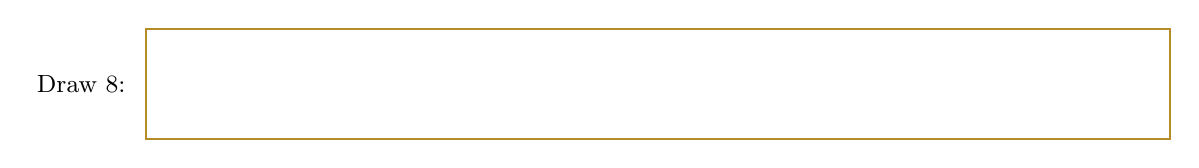
\begin{tikzpicture}
  \draw[thick, scholagold] (0,0) rectangle (13, 1.4);
  \node[left=4pt] at (0,0.7){\small Draw 8:};
\end{tikzpicture}

\bigskip
\noindent\textbf{6.} $6 - 4 = $ \numbox

\medskip
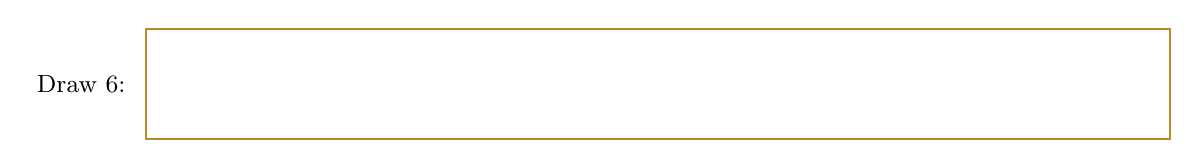
\begin{tikzpicture}
  \draw[thick, scholagold] (0,0) rectangle (13, 1.4);
  \node[left=4pt] at (0,0.7){\small Draw 6:};
\end{tikzpicture}

\bigskip
\noindent\textcolor{scholared}{\rule{\linewidth}{0.4pt}}

% ===== PART III: STORY PROBLEMS =====
\noindent\textcolor{scholared}{\large\textbf{Part III — Story Problems}} \hfill \textit{(Problems 7–10)}

\bigskip

\begin{storybox}
\textbf{7.} Jemima had 9 eggs in her nest. A fox took 3. How many eggs are left?\\[6pt]
\hspace{1em} $9 - 3 = $ \numbox
\end{storybox}

\bigskip

\begin{storybox}
\textbf{8.} There were 10 tadpoles in the pond. 4 became frogs and hopped out.\\
How many tadpoles are left?\\[6pt]
\hspace{1em} $10 - 4 = $ \numbox
\end{storybox}

\bigskip

\noindent\textbf{9.} $8 - 5 = $ \numbox \hspace{2cm}
\textbf{10.} Write your own subtraction story below, then solve it.

\medskip
\hspace{1em} \biganswerline

\medskip
\hspace{1em} \numbox \; $-$ \; \numbox \; $=$ \; \numbox

\end{document}
